\chapter{Сервис балансировки ProWD}
\label{ch:prowd}

\begin{marginfigure}[0.0cm]
{
\setlength{\fboxsep}{0pt}%
\setlength{\fboxrule}{1pt}%
\fcolorbox{gray}{gray}{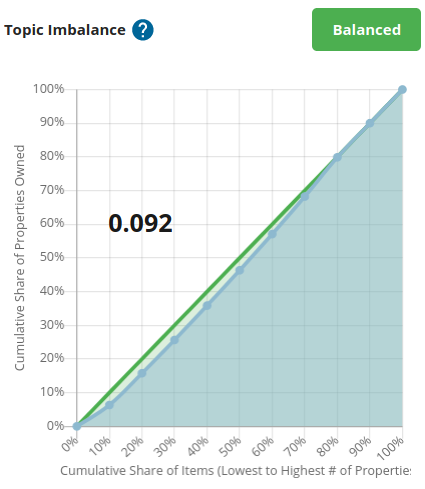
\includegraphics{./chapter/prowd/ProWD-green-balance_Country.png}}
}
  \caption{Высокая степень равномерности заполнения по числу свойств объекта Викиданных 
                \href{https://www.wikidata.org/wiki/Q6256}{страна (Q6256)}. 
                Данные получены с помощью сервиса ProWD.id, 2020 год.
                \emph{Коэффициент Джини равен 0.092.}}%
  \label{fig:prowd_green-balanced}%
\end{marginfigure}

\begin{marginfigure}[0.0cm]
{
\setlength{\fboxsep}{0pt}%
\setlength{\fboxrule}{1pt}%
\fcolorbox{gray}{gray}{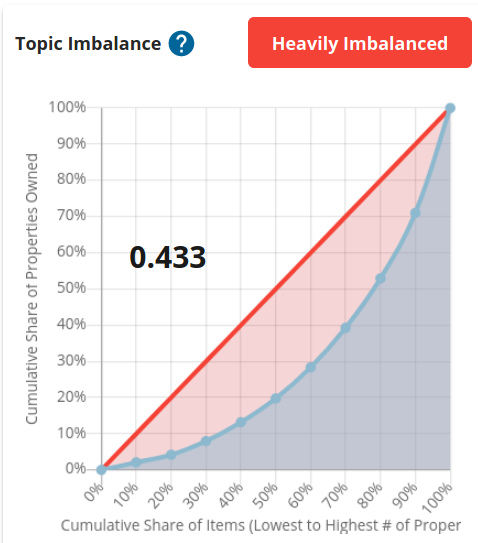
\includegraphics{./chapter/prowd/ProWD-red-imbalance_programming_language_2020-10-09.png}}
}
  \caption{Низкая степень равномерности заполнения свойств у языков программирования (Q9143) по Викиданным на 2020 год.
  \emph{Коэффициент Джини равен 0.433.}}%
  \label{fig:prowd_red-imbalanced}%
\end{marginfigure}



\ifnumequal{\value{draft}}{1}{%
    \todo[inline]{Todo: Что такое <<сбалансированное дерево>> в дискретной математике? Рисунок?\newline 
        Какие могут быть <<перекосы>> при заполнении данных?\newline
        Неравномерность заполнения данных в Википедии? Почему? На примере архивов в ВД.}
}% eo draft

С помощью сервиса ProWD можно анализировать объекты Викиданных. 
Взяв любой объект, например, \wdqName{<<архив>>}{166118}, можно увидеть: 
\begin{itemize}
    \item какой архив мира наиболее проработан по числу свойств,

    \item значение \href{https://w.wiki/gg7}{коэффициента Джини}, 
        показывающего насколько равномерно по числу свойств заполнены <<архивы>>, то есть экземпляры объекта <<архив>>. 
        На полях приведены два рисунка, полученные с помощью сервиса ProWD. 
        На рис.~\ref{fig:prowd_green-balanced} показана высокая степень 
        равномерности заполнения свойств у стран на Викиданных. 
        Это можно объяснить важностью объектов-стран и тем, что 
        сотни пользователей многих википедий их редактируют.
        На рис.~\ref{fig:prowd_red-imbalanced} видно, что 
        у объектов <<языки программирования>> число свойств распределено неравномерно. 
        Есть небольшое число языков, у которых заполнено максимальное число свойств, 
        но у подавляющего большинства языков-объектов заполнено мало свойств.

    \item можно сравнить подклассы объекта по количеству свойств. 
        В статье Elisabeth Giesemann\autocite{Giesemann2020} 
        с помощью сервиса ProWD сравнивают мужчин и женщин, специалистов в области информатики.
\end{itemize}




%\begin{figure}
%{%
%\setlength{\fboxsep}{0pt}%
%\setlength{\fboxrule}{1pt}%
%\fcolorbox{gray}{gray}{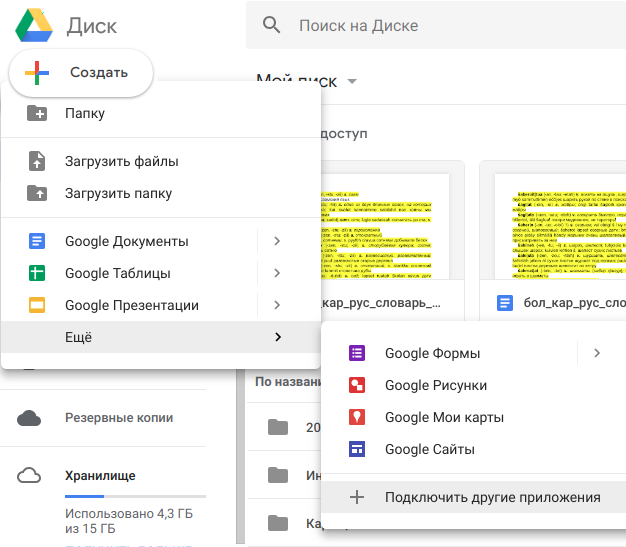
\includegraphics{./lessons/db_google_fusion/020_google_drive_connect_more_apps_with_new-button_ru.png}}%
%}%
%    \caption[Подключения приложения к Google Диску.][56pt]{Подключения 
%            приложения к Google Диску.
%    }
%  \label{fig:google_drive_connect_more_apps}
%\end{figure}


